\section{Discussion}
\label{sec:limitations}
% ══════════════════════════════════════════════════════════════

\textbf{Scope of the evidence.}
The results should be read as a stress test of model-induced rankings under a fixed information set.
The fixed 30-stock NASDAQ panel, short post-release windows, simplified shorting assumptions, and possible hidden memorization channels limit direct claims about deployable trading performance.
Their value is instead diagnostic: the same protocol reveals which LLMs induce monotone rankings, positive IC, distinct style loadings, and residual alphas under conservative timing.

\textbf{Model generation effect.}
The most striking finding is the gap between generations and vendors: within OpenAI, o3's expected-return IC of 0.594 and GPT-4.1's 0.549 greatly exceed GPT-4o's 0.090 and GPT-4o mini's $-0.303$; within Google, Gemini 2.5 Pro and Flash both deliver strong positive ICs despite short conservative windows.
The pattern is directionally consistent with model capability: newer reasoning models and larger frontier models tend to produce stronger rankings, although price is not a sufficient statistic because smaller models such as Gemini 2.5 Flash and GPT-4.1 mini remain competitive.

\textbf{Ranking vs.\ classification.}
Full rankings expose signal structures that classification would hide: GPT-4o mini's \emph{anti-monotonic} quintile returns would be invisible under a 5-category Buy/Hold/Sell scheme, and o3's market-neutral long--short Sharpe of 5.54 is only attainable when rankings separate both the top and bottom of the cross-section.
In our setting, the bottom quintile is as informative as the top: strong models avoid the same stocks that weak models over-rank, converting a long-only selection signal into an investable spread.
Buy/Hold/Sell labels or top-$k$ hit rates would therefore understate both positive and negative model skill.

\textbf{Cost--effectiveness and reproducibility.}
Gemini 2.5 Flash, GPT-4.1 mini, and GPT-4.1 nano offer strong cost--performance trade-offs among included models: all are inexpensive relative to larger frontier or reasoning models yet deliver positive spreads after conservative-window filtering.
High-cost models such as Claude Opus 4 are less attractive on a spread-return basis.
The relevant unit is not leaderboard capability but ranking quality per dollar under a fixed information set.

\begin{figure}[H]
  \centering
  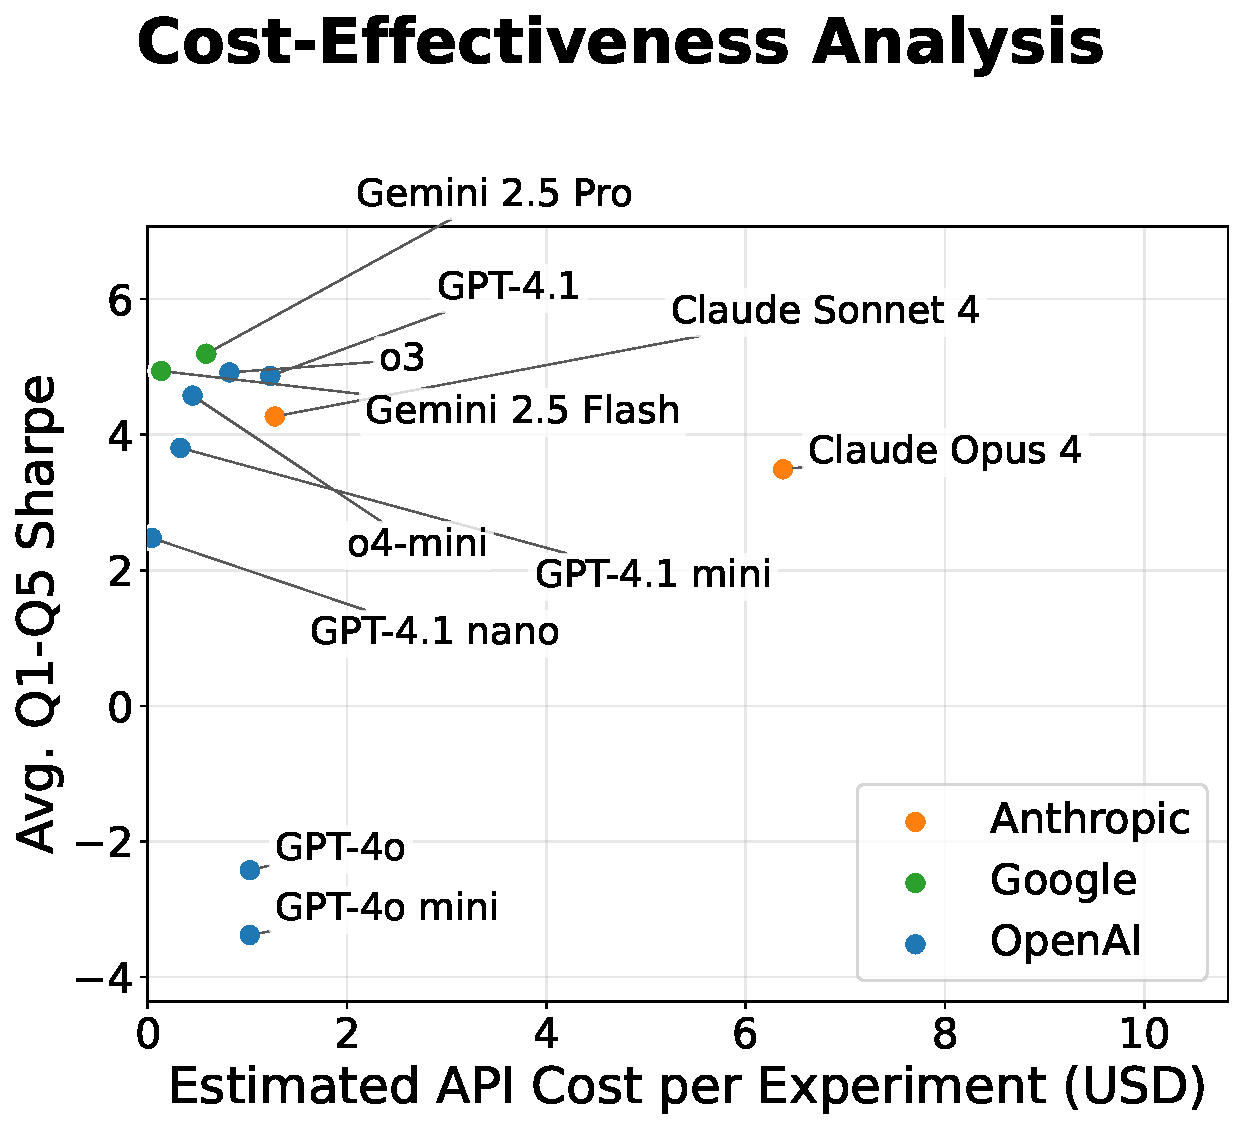
\includegraphics[width=0.92\columnwidth]{figures/fig5_cost_effectiveness.pdf}
  \caption{Cost versus average Q1$-$Q5 Sharpe for tested LLM rankers.}
  \Description{Scatter plot comparing model cost with average long-short Sharpe, with vendor colors and labels showing that several lower-cost OpenAI and Google models lie near the efficient frontier.}
  \label{fig:cost-main}
\end{figure}

Cost should be reported at the experiment level rather than only per token because pairwise or agentic variants can multiply API usage quickly.

\textbf{Risk-adjusted prompts as implicit risk control.}
Prompting for Sharpe/Sortino acts as implicit risk control even without weights or an optimizer: the risk-adjusted objectives often reduce drawdowns or change which names enter Q1 and Q5.
The factor analysis (Section~\ref{sec:factor}) confirms a genuine style shift, moving the implicit style away from a pure ``momentum $\times$ growth'' profile toward more risk-aware rankings for some models.
However, the risk prompts do not uniformly improve ranking quality.
They often reduce drawdowns by dampening the high-momentum growth tilt, but they can also dilute or redirect the strongest return signal, as seen in the model-specific differences between expected-return, Sharpe, and Sortino prompts.
Prompt choice should therefore be viewed as a style-control knob rather than a free improvement in objective alignment.

\textbf{IC as diagnostic, vendor risk profiles, and limitations.}
Mean IC and long--short Sharpe are near-linearly related ($r = 0.90$, $p<0.001$), making IC a reliable ex-ante diagnostic.
Anthropic long--short portfolios show relatively shallow drawdowns in conservative windows, while the GPT-4o family shows much deeper losses and negative ICs.
Remaining limitations are important for follow-on work: post-cutoff windows reduce direct leakage from evaluated holding-period returns, but broader LLM memorization, hidden lookahead channels \citep{gao2025lookahead,merchant2025lookahead}, and market reflexivity in historical AI backtests \citep{koijen2026agentic} warrant formal testing; backtest windows differ outside the common-window robustness check; and LLM outputs can drift across API versions despite temperature $=0$.
Some historical model IDs are preview, date-pinned, or currently unavailable for live reruns, so we distinguish cached benchmark evidence from future live-API reproducibility.
We therefore interpret the results as a controlled model-comparison benchmark rather than evidence of production tradability.
A natural benchmark extension is to add pointwise LLM scoring, pairwise or setwise tournaments, ensembles, and lightweight agentic rankers on the identical information set.
The fixed listwise protocol isolates a minimum viable cross-sectional ranker before adding retrieval, debate, tool use, or portfolio optimization layers.
Negative results are equally informative: GPT-4o mini persistently ranks the cross-section in the wrong direction, producing negative IC and anti-monotonic quintiles rather than merely noisy alpha.
For benchmark design, rank IC, portfolio spreads, and style diagnostics should therefore be reported together: IC tests ordering quality, spreads test economic investability, and factor diagnostics test whether apparent alpha is just familiar style compensation.

% ══════════════════════════════════════════════════════════════
